% === Fig. 1: Diagnostic Summary ===
\begin{figure*}[t]
    \centering
    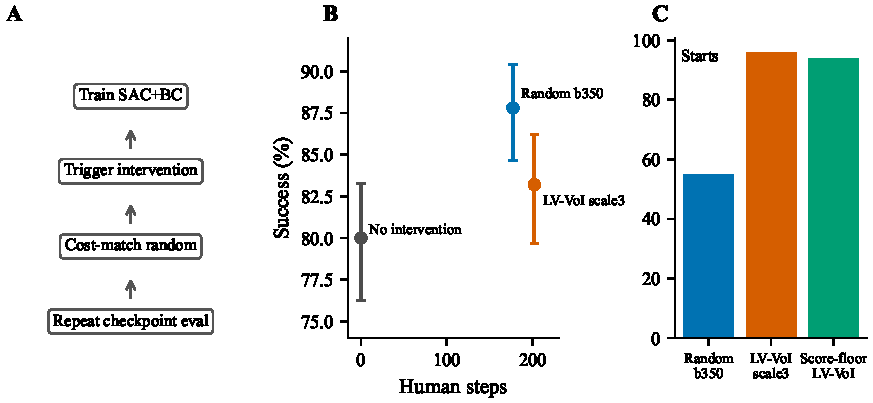
\includegraphics[width=0.95\textwidth]{figures/fig1_hero_diagnostic_summary.pdf}
    \caption{Diagnostic evaluation pipeline and main failure pattern. Cost matching reverses the initially promising LV-VoI result, and trace diagnostics reveal over-triggering rather than simple far-from-object intervention.}
    \label{fig:diagnostic_summary}
\end{figure*}

% === Fig. 2: Cost-Matched Frontier ===
\begin{figure}[t]
    \centering
    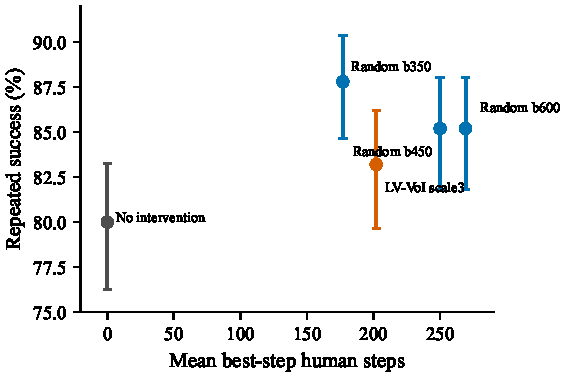
\includegraphics[width=0.48\textwidth]{figures/fig2_cost_matched_frontier.pdf}
    \caption{Cost-matched Lift frontier over five seeds. The lower-budget random baseline dominates LV-VoI scale3 in both repeated success and best-step human cost.}
    \label{fig:cost_matched_frontier}
\end{figure}

% === Fig. 3: Trigger Repairs ===
\begin{figure}[t]
    \centering
    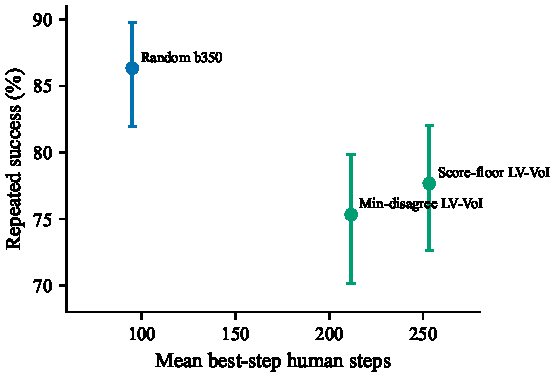
\includegraphics[width=0.48\textwidth]{figures/fig3_trigger_repairs.pdf}
    \caption{Two intuitive trigger repairs remain dominated by same-seed random intervention.}
    \label{fig:trigger_repairs}
\end{figure}

% === Fig. 4: Intervention Timing ===
\begin{figure}[t]
    \centering
    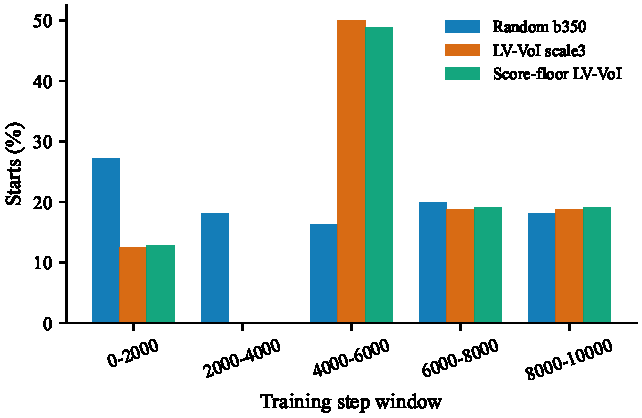
\includegraphics[width=0.95\textwidth]{figures/fig4_intervention_timing.pdf}
    \caption{Intervention-start timing distribution. LV-VoI variants concentrate starts in the mid-run window and use more starts than random.}
    \label{fig:intervention_timing}
\end{figure}

% === Fig. 5: Score Over Time ===
\begin{figure}[t]
    \centering
    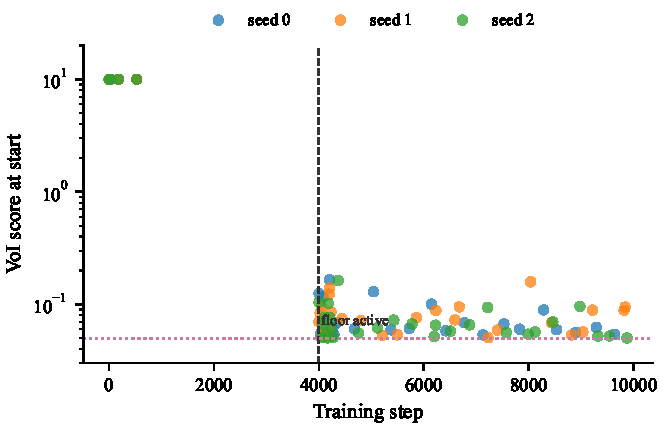
\includegraphics[width=0.95\textwidth]{figures/fig5_score_over_time.pdf}
    \caption{R024 score-floor diagnostics. The floor blocks sub-threshold starts after step 4000, but accepted scores remain frequent enough to consume nearly the full budget.}
    \label{fig:score_over_time}
\end{figure}
